%==============================================================================
%== template for LATEX poster =================================================
%==============================================================================
%
%--A0 beamer slide-------------------------------------------------------------
\documentclass[final]{beamer}
\usetheme[secheader]{Boadilla}
\usepackage[orientation=portrait,size=a0,
	scale=1.25				 % font scale factor
	]{beamerposter}

\addtobeamertemplate{block example begin}{%
	\setlength{\textwidth}{0.31\textwidth}%
}{}
\addtobeamertemplate{block begin}{%
	\setlength{\textwidth}{0.31\textwidth}%
}{}

\geometry{
	hmargin=2.5cm, % little modification of margins
	tmargin=2.5cm,
}

%
\usepackage[utf8]{inputenc}
\usepackage{tabularx}
\usepackage{textcomp}
\usepackage{tikzsymbols}

\usepackage{tikz}
\usetikzlibrary{mindmap}

\usepackage{smartdiagram}
\tikzset{priority arrow/.append style={
	rotate=180,
	anchor=0,
	xshift=30,
	}
}
\smartdiagramset{
priority arrow width=2cm,
priority arrow height advance=3cm,
priority tick size=10pt,
}
\smartdiagramset{
	descriptive items y sep=2.5cm,
	description width=8cm,
	description text width=8cm,
}

\linespread{1.2}

\usepackage{caption}
\captionsetup{justification=raggedright,singlelinecheck=false}
\usepackage{newfloat}
\DeclareFloatingEnvironment[fileext=diag,placement={!ht},name=Diagram]{diag}
%
%==The poster style============================================================
\usetheme{sharelatex}

%==Title, date and authors of the poster=======================================
\title
[7th International Congress of the Molecular Biology Association of Turkey, 27 - 29 September 2019, İstanbul, Turkey] % Conference
{ % Poster title
	PICUS: \textbf{P}ointed \textbf{I}nterpretation of \textbf{C}linical \textbf{V}ariant \textbf{S}ignificance
}

\author{ % Authors
Barış Salman\inst{1,2}, Sibel Uğur İşeri\inst{2}
}
\institute
[Very Large University] % General University
{
\inst{1} Gen-Era Diagnostics, Bioinformatics Department\\[0.3ex]
\inst{2} İstanbul University, Aziz Sancar DETAE
}
\date{\today}

\begin{document}
\begin{frame}[t]
%==============================================================================
\begin{multicols}{3}
%==============================================================================
%==The poster content==========================================================
%==============================================================================

\section{Introduction}

Analyses of genetic variations have identified molecular basis for over 5000 diseases
through the past decades \cite{omim}. Growing knowledge on inherited diseases and
gradual decrease in the cost of next generation sequencing (NGS) applications have made
NGS based genetic tests feasible for genetic diagnosis. However, the emergence of NGS
in the era of clinical genetics comes with various challenges. One of those challenges is
assessing the significance of genetic variations in the human genome.
American College of Medical Genetics and Genomics (ACMG) and
the Association for Molecular Pathology (AMP) guide has been widely used as standard
for sequence variant interpretation regarding 28 criteria \cite{acmg}
based on various attributes of the given variant (Table \ref{ACMGtable}).
However, there is significant variance when it comes to	implementations of those criteria
among different institutes and genome analysts. We have therefore set out to automatize
ACMG/AMP criteria via developing a novel bioinformatics tool, namely ‘picus’\cite{aeneid}.

\vskip1ex
\begin{table}
\centering
\caption{ACMG/AMP criteria breakdown in 8 categories}
\label{ACMGtable}
\begin{tabularx}{0.3\textwidth}{X X X}
\hline\hline
\ & Pathogenic & Benign \\
\hline
	Population Data & PS4 PM2 & BA1 BS1 BS2 \\
	Comp. and Pred. Data & PP3 & BP4 BP7 \\
	Functional Data & PVS1 PS3 PM1 PM4 PP2 & BS3 BP1 BP3 \\
	Segregation Data & PP1 & BS4 \\
	De Novo Data & PS2 PM6 & \\
	Allelic Data & PM3 & BP2 \\
	Other Database & PS1 PM5 PP5 &	BP6 \\
	Other Data & PP4 & BP5 \\
\hline\hline
\end{tabularx}
\end{table}
\vskip2ex

\small
\textbf{Keywords: Next generation sequencing, medical genetics, bioinformatics, automation of ACMG/AMP criteria}
\normalsize

\section{Result \& Discussions}
\begin{block}{}
Picus v0.0.4 can automate interpretation of 13 ACMG/AMP criteria
in order to classify variants based on significance. There is still need
for further manual interpretation in order to incorporate individual of
family specific metrics such as segregation data and de novo status of variants.
\end{block}

Research projects have the advantage of selecting desired number of samples
from well phenotyped cohorts. Pace of the study is mostly set by publishing
papers and various genomic and other experimental methods can be used when
assessing a variants significance. More related individuals can be gathered
from the family to increase the statistical power (Table \ref{RRtable}).

\vskip1ex
\begin{table}
\centering
\caption{Research vs Routine}
\label{RRtable}
\begin{tabularx}{0.3\textwidth}{X X X}
\hline\hline
\ & Research & Routine \\
\hline
	Pace & Slow & Fast \\
	Sample Volume & Low & High \\
	Methods & Various & Restricted \\
	Families & Large & Small \\
\hline\hline
\end{tabularx}
\end{table}
\vskip2ex

In contrast most of the above cannot or may not be carried out in clinical setting. Because;
\begin{block}{}
\begin{itemize}
\item Patients are phenotypically heterogeneous.
\item There are no cap in number of patients.
\item Mostly it is not possible to include any members further than nuclear family members.
\item In vivo/vitro methods are restricted since it takes extra time, energy, budget and a team of specialized people.
\end{itemize}
\end{block}

Software packages that streamline any static and repetitive part of clinical
process saves time that can be used to better evaluate the situation. Picus
streamlines the process of evidence collection and allows more time to be spent
evaluating variants based on their idiosyncratic features (Figure \ref{Varint}). As a result aiming
to lower the number of variants of unknown significance that cause a halt in
clinical process and adverse psychological effects on patients\cite{vus}.

\vskip10ex
\begin{center}
\begin{figure}
\caption{Solving human disease}
\label{Varint}
\hspace*{-4cm}
\begin{tikzpicture}[mindmap, grow cyclic, every node/.style=concept, text width=,minimum size=6cm, concept color=orange!40,
	level 1/.append style={level distance=9cm,sibling angle=120},
	level 2/.append style={level distance=7cm,sibling angle=90},]
\node{Human Disease}
child [concept color=blue!30, text width=,minimum size=4cm] { node {Clinical Genetics}
	child [text width=,minimum size=2cm] { node {Diagnosis}}
	child [text width=,minimum size=2cm] { node {Screening}}
	child [text width=,minimum size=2cm] { node {Counseling}}
}
child [concept color=purple!50, text width=,minimum size=4cm] { node {Genomics}
	child [text width=,minimum size=2cm] { node {Molecular Genetics}}
	child [text width=,minimum size=2cm] { node {Population Genetics}}
	child [text width=,minimum size=2cm] { node {Functional Genetics}}
}
child [concept color=teal!40, text width=,minimum size=4cm] { node {Bioinformatics}
	child [concept color=green!40, text width=,minimum size=2cm] { node {Variant Interpretation}}
	child [text width=,minimum size=2cm] { node {Variant Filtering}}
	child [text width=,minimum size=4cm] { node {NGS}}
};
\end{tikzpicture}
\end{figure}
\end{center}

\section{Material \& Method}

Picus is developed using Python with the Pandas\cite{pandas} module.
After processing raw fastq data into variant call format (vcf),
vcf is further annotated using Ensembl Variant Effect Predictor\cite{vep} (VEP) tool (Diagram \ref{workflow}).
Parameters such as disease and allele frequency, domain structure of proteins,
in silico prediction metrics and documented variant data retrieved from ClinVar
have been used for automatized processing of ACMG/AMP criteria prediction.
As a result, each variant can be classified as pathogenic, likely pathogenic,
benign, likely benign or uncertain significance as suggested by ACMG/AMP.

\begin{center}
\captionof{diag}{Sequence variant discovery workflow}
\label{workflow}
\scalebox{1.3}{
\smartdiagram[priority descriptive diagram]{
	Interpretation \large \Strichmaxerl \normalsize,
	Classification (Picus),
	Annotation (VEP),
	Filter Variants (Dove),
	Fastq\textrightarrow Vcf (Pigeon),
	NGS Platform
}
}
\end{center}

\subsection{How to use}

Picus can be run anywhere with a python3 interpreter and can be installed
with pip (See project page\cite{github}). Help screen can be viewed with
command 'picus -h' that summarizes parameters (Figure \ref{picushelp}).

\begin{center}
	\begin{figure}
		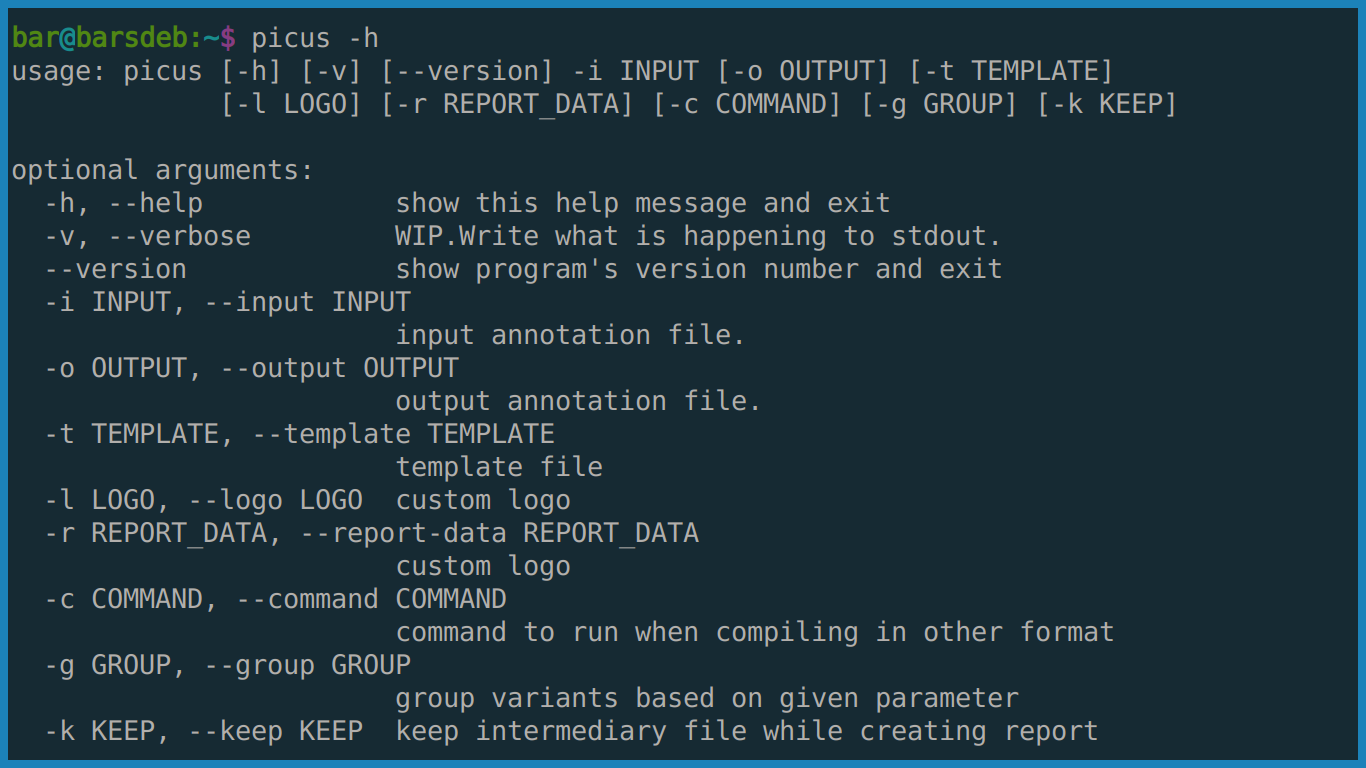
\includegraphics[width=\linewidth]{picus_help.png}
		\caption{Picus help screen}
		\label{picushelp}
	\end{figure}
\end{center}

Analysis can be carried out after Vcf is VEP annotated with following command.

\vskip2ex
\begin{columns}
	\begin{column}{0.01\textwidth}
	\end{column}
	\begin{column}{0.99\textwidth}\centering
	\begin{exampleblock}{Usage example}
		\vskip1ex
		picus -i sample.VEP.tsv -o sample.VEP.picus.tsv
	\end{exampleblock}
		\end{column}
\end{columns}
\vskip4ex

\section{Summary \& Conclusions}

\begin{block}{}
There is high demand for customized bioinformatic tools that could be used in
the medical genetics area due to growing number of NGS based genetic tests under clinical setting.
Picus aims to help genome analysts in this concept via increased automation in ACMG/AMP criteria.
\end{block}

%==============================================================================
%==End of content==============================================================
%==============================================================================

%--References------------------------------------------------------------------

\subsection{References}

\begin{thebibliography}{99}

\footnotesize
\renewcommand{\baselinestretch}{.2}
\bibitem{omim} \url{https://omim.org/statistics/entry}
\bibitem{acmg} Richard S., et. al., Standards and guidelines for the interpretation of sequence variants: a joint consensus recommendation of the American College of Medical Genetics and Genomics and the Association for Molecular Pathology \textit{Genetics in Medicine}, 2015
\bibitem{aeneid} http://classics.mit.edu/Virgil/aeneid.7.vii.html
\bibitem{vus} Makhnoon S., et. al., Experiences of patients seeking to participate in variant of uncertain significance reclassification research, \textit{Journal of Community Genetics}, 2019
\bibitem{pandas} McKinney W., Data Structures for Statistical Computing in Python, \textit{Proceedings of the 9th Python in Science Conference}, 2010
\bibitem{vep} McLaren W., The Ensembl Variant Effect Predictor, Genome Biology, 2016
\bibitem{github} https://github.com/barslmn/picus
\normalsize

\end{thebibliography}
%--End of references-----------------------------------------------------------

\footnotesize
% \subsection{About name}
% \begin{verse}
% For Circe long had lov'd the youth in vain,\\
% Till love, refus'd, converted to disdain:\\
% Then, mixing pow'rful herbs, with magic art,\\
% She chang'd his form, who could not change his heart;\\
% Constrain'd him in a bird, and made him fly\cite{aeneid}
% \end{verse}

\end{multicols}

%==============================================================================
\end{frame}
\end{document}
